\documentclass[a4paper,11pt]{article}

\usepackage[utf8]{inputenc}
\usepackage[italian]{babel}
\usepackage{geometry}
\usepackage{graphicx, wrapfig}
\usepackage{multicol} % Used for the two-column layout of the document
\usepackage{amsmath}
\usepackage{caption}
\usepackage[a-1b]{pdfx}

\newgeometry{vmargin={10mm,28mm}, hmargin={25mm,25mm}}

\hypersetup{%
    pdfpagemode={UseOutlines},
    bookmarksopen,
    pdfstartview={FitH},
    colorlinks,
    linkcolor={black}, %COLORE RIFERIMENTI INDICE
    citecolor={blue}, %COLORE CITAZIONI
    urlcolor={blue}, %COLORE URL
}

% Definition of \maketitle
\makeatletter
\newcommand{\departmentname}[1]{\def\@departmentname{#1}}
\newcommand{\coursename}[1]{\def\@coursename{#1}}
\newcommand{\academicyear}[1]{\def\@academicyear{#1}}
\newcommand{\advisorname}[1]{\def\@advisorname{#1}}
\newcommand{\coadvisorname}[1]{\def\@coadvisorname{#1}}
\newcommand{\studentname}[1]{\def\@studentname{#1}}
\newcommand{\itathesistitle}[1]{\def\@itathesistitle{#1}}
\newcommand{\engthesistitle}[1]{\def\@engthesistitle{#1}}

\def\@maketitle{
	\begin{center}
		
\includegraphics[width=4cm]{images/logoUnipr.png}\\[2ex]
		\@departmentname\\[1ex]
		\@coursename\\
		\noindent\rule{8cm}{0.4pt}\\[1ex]
		\@itathesistitle\\[1ex]
		\@engthesistitle
	\end{center}
	\underline{Relatore:}
	\hfill
	\underline{Tesi di Laurea di:}\\
	\@advisorname
	\hfill
	\@studentname\\[1ex]
	\underline{Correlatore:}\\
	\@coadvisorname
	\begin{center}
		\@academicyear
	\end{center}
	\vskip 0.1cm
}
\makeatother

\departmentname{\textbf{Dipartimento di Ingegneria e Architettura}}
\coursename{\textbf{Corso di Laurea Triennale in Ingegneria Informatica}}
\academicyear{ANNO ACCADEMICO 2019/2020}
\advisorname{Prof. Michele Amoretti}
\coadvisorname{Prof. Andrea Prati}
\studentname{Daniele Pellegrini}
\itathesistitle{Refactoring di un Software per la Prenotazione di Servizi Sanitari}
\engthesistitle{Refactoring of a Software for Booking Healthcare Services}

\begin{document}
	\maketitle
   	%\lipsum
	   Il progetto di Tesi descritto in questo elaborato ha come obiettivo la reingegnerizzazione di un software utilizzato per la prenotazione di servizi sanitari: \emph{Zerocoda}. L'elaborato presentato è un elaborato di tirocinio svolto presso l'azienda \emph{Maps Group S.p.A} totalmente in loco, presso la sede centrale. Il tirocinio, oltre ai fini di curriculum, è stato svolto per permettermi di interfacciarmi per la prima volta con la quotidianità del mondo del lavoro in un contesto completamente nuovo: quello aziendale. L'azienda si occupa principamente si sviluppo software, vantando diversi clienti riconosciuti a livello nazionale.
	   
	   L'applicativo permette, a seconda della struttura ospedaliera presso cui si prenota, di usufruire di diverse tipologie di servizi. Il primo scopo di questa applicazione è quello di velocizzare l'accesso ai servizi, controllandone l’affluenza. I benefici derivanti da questo refactoring non sono limitati al cliente, che in questo modo può continuare a prenotarsi nell'orario che desidera, ma riguardano anche la struttura. Essa infatti, attraverso una corretta implementazione del software, migliora il sistema logistico. Avere a disposizione con largo anticipo i dati dell'utente prenotato, significa avere anche la possibilità di preparare l'occorrente della visita medica per tempo. Oltre alla riduzione del contatto interpersonale, l’ottimizzazione di software come questo può ridurre il rischio di assembramento e una migliore profilazione dell’utente con cui il personale e gli altri clienti entrano in contatto. Il COVID19 ha portato questa esigenza, che inizialmente era una comodità, ad essere a tutti gli effetti una necessità e un requisito fondamentale per le aziende che richiedono questo tipo di servizi: per la loro gestione interna e per garantire la sicurezza dei loro clienti, a maggior ragione per quelle nel settore sanitario. 
	   
	   Nel primo capitolo dell'elaborato sono state presentate le tecnologie utilizzate per la risoluzione del problema, giustificando le scelte fatte.  Si è proceduto con un'azione di reverse engineering del sistema, dove sono stati analizzati i suoi punti critici. Infine si è passati alla progettazione del nuovo sistema, in particolare allo studio di una soluzione sulla base dei dati raccolti e alla sua successiva implementazione. Nell'ultimo capitolo sono stati svolti degli \emph{stress test} sul sistema di partenza e quello implementato, mettendo a confronto i risultati ottenuti. In queste fasi non si è agito direttamente sul frontend, la parte visibile dall’utente finale e con la quale interagisce, ma sul backend, la parte del sistema che elabora i dati e che ha il compito di interfacciarsi con il database, dove questi vengono salvati. Il fine ultimo di quest’opera di reingegnerizzazione è stata la costruzione di un nuovo layer di REST APIs dietro un reverse proxy. Il sistema di partenza non presenta un layer di API, pertanto le chiamate dal frontend al backend vengono trasmesse in modo contorto e poco efficiente: la banalità del sistema monolitico può essere causa di un attacco informatico o malfunzionamenti, per questo si è optato per un’architettura di microservizi.

	\begin{figure}
		\centering
		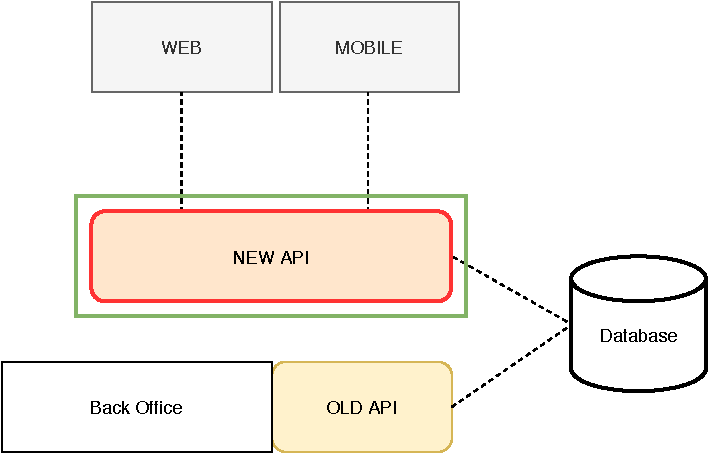
\includegraphics[width=0.90\textwidth]{images/01_nuove_api.pdf}
	\end{figure}
	Questo nuovo strato è stato affiancato al sistema esistente, fino a quando un successivo sviluppo ne permetterà una completa migrazione. In Figura viene mostrato come i due sistemi sono disposti a livello architetturale una volta che le nuove API sostituiranno il relativo codice sul branch di produzione. Le vecchie API rimarranno in supporto al backoffice, che sarà oggetto di una fase successiva di refactoring. Per la riscrittura del backend, precedentemente scritto in PHP, è stato utilizzato il linguaggio Java, facendo uso della JDK 15 e del framework Spring. Con la reingegnerizzazione il sistema ottiene nuove funzionalità richieste dalle strutture affiliate e migliora quelle già implementate, il tutto rimanendo coerente con il suo funzionamento: il nuovo strato inserito tra frontend e backend deve infatti garantire il corretto funzionamento di tutte le operazioni che già erano presenti. Sulla base di \emph{Zerocoda}, si è deciso di creare un’applicazionea analoga per i servizi commerciali: \emph{Royalty Zerocoda}. Si tratta di un’esigenza diversa, ma vicina alla precedente. L’idea è già stata sviluppata partendo da un branch di questo software. Il layer di API realizzato costituisce quindi il primo passo sulla strada che porterà alla fusione delle due.
	Al completamento dell'implementazione delle nuove REST APIs seguiranno le successive fasi del refactoring. Queste interessano prima l'Authentication Server, il cui sviluppo è cominciato in parallelo a questo progetto e il frontend, che subirà un leggero restyling finalizzato a migliorare il supporto alle nuove chiamate REST. in seguito si procederà allo sviluppo dell'Authentication Server. Zerocoda offre la possibilità ai propri utenti di essere notificati attraverso email e sms, servizi offerti da enti esterni che permettono all'utente di ricevere aggiornamenti rigurardo lo stato della propria prenotazione o del proprio profilo. L'ultimo parte del refactoring riguarderà il database, dove il sistema di gestione dei dati verrà completamente rivoluzionato rispetto lo stato attuale. A questa modifica seguiranno le correzioni agli elementi a cui si è appena fatto riferimento, che sono stati implementati prima di esso. 

   	\end{document}